\begin{figure}[h]
    \centering
    \noindent\begin{minipage}{.45\linewidth}
        \resizebox{\linewidth}{!}{%
            \begin{tabular}{l|lll}
             & Féminin & Jeunesse & Royal \\ \midrule
            Homme                          & 0       & 0        & 0     \\
            Femme                          & 1       & 0        & 0     \\
            Garçon                         & 0       & 1        & 0     \\
            Fille                          & 1       & 1        & 0     \\
            Prince                         & 0       & 1        & 1     \\
            Princesse                      & 1       & 1        & 1     \\
            Reine                          & 1       & 0        & 1     \\
            Roi                            & 0       & 0        & 1     \\
            Monarque                       & 0.5     & 0.5      & 1    
            \end{tabular}%
        }
    \end{minipage}
    \begin{minipage}{.45\linewidth}
        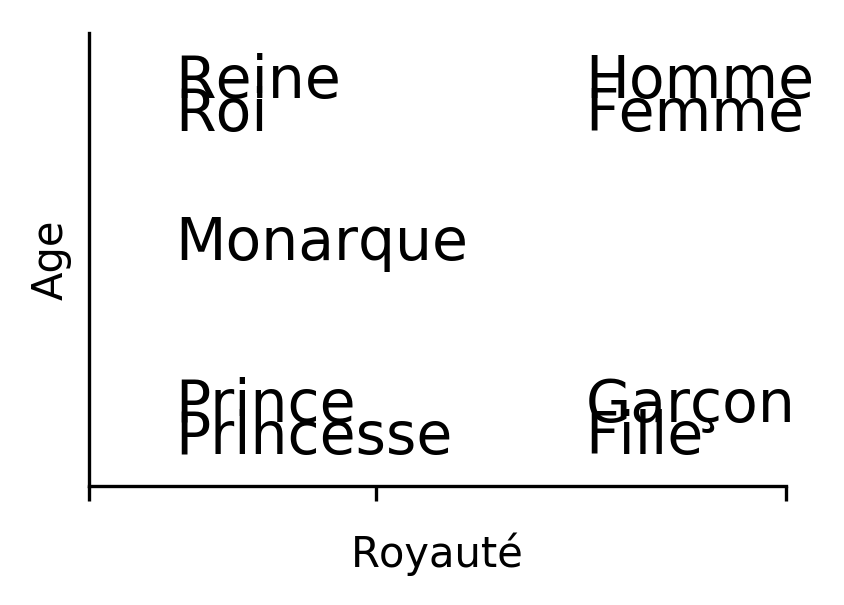
\includegraphics[width=\linewidth]{results/deep-learning/explanations/visualisation_embedding.png}
    \end{minipage}
    \caption{En choisissant des catégories adaptées, il est possible de placer dans un tableau tout un ensemble d'informations et de différencier des éléments de vocabulaire mathématiquement. Ici, \textit{monarque} est neutre, il n'est donc ni féminin (1) ni masculin (0). Une fois ces catégories choisies, on peut les représenter sur deux dimensions via PCA. On remarque alors que les groupes se rassemblent. Inspiration: \cite{lynn_get_2018}}
    \label{figure:deep-learning:projection-embedding}
\end{figure}